\begin{titre}[Étude qualitative de fonctions]

\Titre{Description d'un comportement}{4}
\end{titre}


\begin{CpsCol}
\textbf{Variations de fonctions}
\begin{description}
\item[$\square$] Déterminer graphiquement les extremums d’une fonction sur un intervalle.
\item[$\square$] Exploiter un logiciel de géométrie dynamique ou de calcul formel, la calculatrice ou Python pour décrire les variations d’une fonction donnée par une formule.
\end{description}
\end{CpsCol}

\Rec{1}{VF-0-N}

\begin{DefT}{Tableau de variations}\index{Tableau de variations}
Un tableau de variations d'une fonction $f$ est un tableau dans lequel l'étude synthétise
\begin{description}
\item[•] le domaine de définition de $f$ explicitement,
\item[•] les variations de $f$ à l'aide de flèches,
\item[•] les maximum et minimum.
\end{description} 

\begin{tikzpicture}
\tkzTabInit[lgt=2,espcl=3]{ $x$ / 1,$f$  / 2}
{ $0$ ,$3$,$5$}
\tkzTabVar{+/$3$,-/$1$,+/$2$ }
\end{tikzpicture}
\end{DefT}




\mini{
\EPC{1}{VF-2}{Représenter.}

\EPC{1}{VF-5}{Représenter. Raisonner.}
}{
\EPC{1}{VF-3}{Représenter.}
}

\begin{Rq}
La courbe représentative d'une fonction $f$ et le tableau de variations de $f$ correspondent.
\end{Rq}


\begin{DefT}{Variations - Approche visuelle}
Dans un tableau de variations,
\begin{description}
\item[•] Une fonction croissante sur un intervalle est représentée par une flèche qui monte sur cet intervalle.
\item[•] Une fonction décroissante sur un intervalle est représentée par une flèche qui descend sur cet intervalle.
\end{description}
\end{DefT}



\begin{DefT}{Visualisation d'une fonction croissante ou décroissante}\index{Représentation graphique!Fonction croissante, décroissante}
\begin{description}[leftmargin=*]
\item[•] Lorsque, sur un intervalle $I$, la courbe représentative d'une fonction monte sans portion horizontale, on dit que la fonction est \textbf{strictement croissante sur $I$}. Si la courbe représentative possède une portion horizontale, on dit que la fonction est \textbf{croissante sur $I$}.
\item[•] Lorsque, sur un intervalle $I$, la courbe représentative d'une fonction descend sans portion horizontale, on dit que la fonction est \textbf{strictement décroissante sur $I$}. Si la courbe représentative possède une portion horizontale, on dit que la fonction est \textbf{décroissante sur $I$}.
\end{description}
\end{DefT}




\begin{DefT}{Maximum, minimum}
On dit que
\begin{description}[leftmargin=*]
\item[•] $M$ est le maximum de $f$ sur son domaine de définition si pour tout réel $x$ de $I$, $f(x) \leq M$. 
\item[•] $m$ est le minimum de $f$ sur son domaine de définition si pour tout réel $x$ de $I$, $f(x) \geq m$. 
\end{description} 
On dit que $f$ est bornée  sur $I$ lorsque $f$ accepte un maximum \textbf{et} un minimum sur $I$.
\end{DefT}


 \EPC{1}{VF-3bis}{Communiquer.}

\begin{DefT}{Fonction croissante, décroissante sur $I$ - Approche comparatiste}
On dit que
\begin{description}[leftmargin=*]
\item[•] une fonction $f$ est \textbf{croissante sur $I$}, lorsque pour tout nombre $a$ et $b$ de $I$, les images de $a$ et de $b$ sont rangées dans le même ordre que $a$ et $b$.
\item[•] une fonction $f$ est \textbf{décroissante sur $I$}, lorsque pour tout nombre $a$ et $b$ de $I$,  les images de $a$ et de $b$ sont rangées dans l'ordre inverse de $a$ et $b$.
\end{description} 
\end{DefT}

 

\begin{DefT}{Fonction croissante, décroissante sur $I$  - Approche analytique }
\begin{description}[leftmargin=*]
\item[•] une fonction $f$ est \textbf{croissante sur $I$}, lorsque pour tout nombre $a$ et $b$ de $I$ tels que $a \leq b$, $f(a) \leq f(b)$.
\item[•] une fonction $f$ est \textbf{strictement croissante sur $I$}, lorsque pour tout nombre $a$ et $b$ de $I$ tels que $a \leq b$, $f(a) < f(b)$.
\item[•] une fonction $f$ est décroissante sur $I$, lorsque pour tout nombre $a$ et $b$ de $I$ tels que $a \leq b$, $f(a) \geq f(b)$.
\item[•] une fonction $f$ est décroissante sur $I$, lorsque pour tout nombre $a$ et $b$ de $I$ tels que $a \leq b$, $f(a) > f(b)$.
\end{description} 
\end{DefT}

\EPC{1}{VF-4}{Raisonner. Communiquer.}
 
\EPC{0}{VF-29}{Raisonner. Représenter. Communiquer. }






\begin{minipage}{0.47\linewidth}
\EPC{1}{VF-12}{Raisonner. Représenter.}
\end{minipage}
\hfill
\begin{minipage}{0.47\linewidth}
\EPC{0}{VF-13}{Raisonner. Communiquer.}
\end{minipage}


\begin{minipage}{0.5\linewidth}
\EPC{1}{VF-27}{Représenter. Raisonner. }
\end{minipage}
\hfill
\begin{minipage}{0.47\linewidth}
\EPC{1}{VF-7}{Raisonner. Communiquer.}
\end{minipage}

 


\EPC{0}{VF-28}{Raisonner. Communiquer. }



 


%\EPC{1}{VF-28_cor}{Raisonner. Communiquer. }

%\EPC{1}{VF-29_cor}{Raisonner. Représenter. Communiquer. }